\documentclass[11pt]{article}
\usepackage{tikz}
\usepackage{amssymb}
\usepackage{geometry}
\geometry{letterpaper, landscape, margin=0.4in}
\usetikzlibrary{positioning, calc}

\begin{document}

\begin{center}
{\Huge \textbf{THE DEEP SANCTUM}}\\[0.3em]
{\Large Level 3A --- Restless Dead \& The Seal | 16 Keyed Areas}
\end{center}

\vspace{0.3em}

\begin{center}
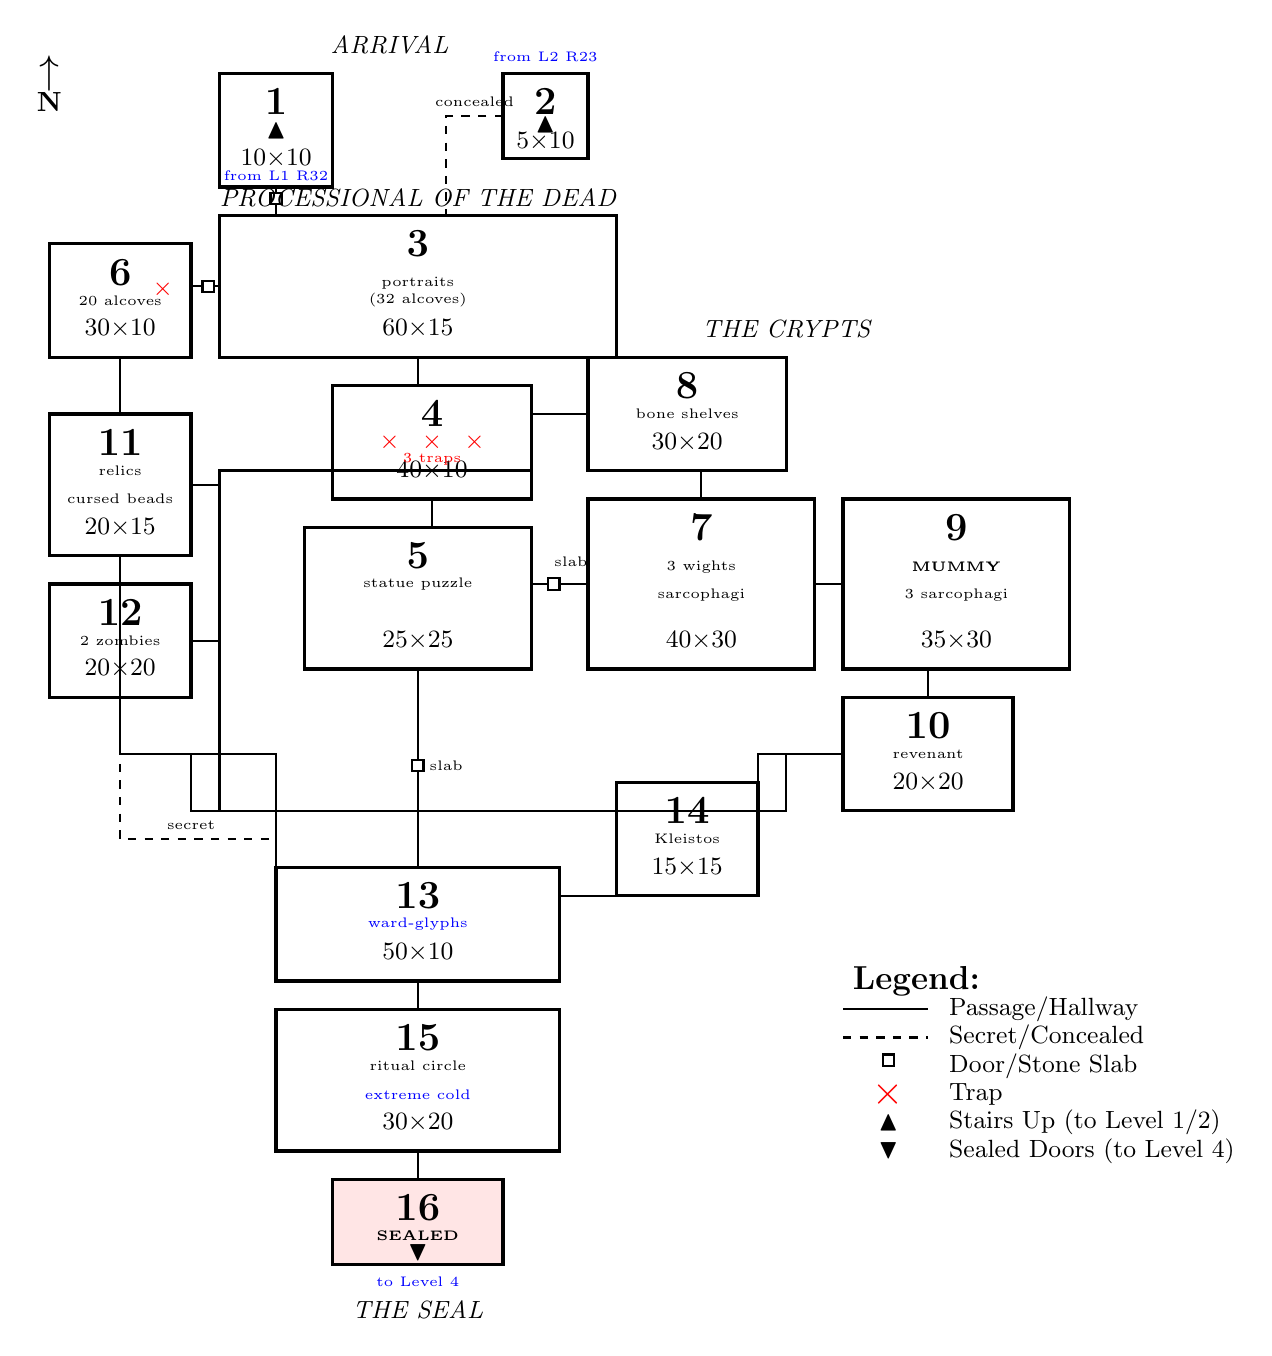
\begin{tikzpicture}[
    room/.style={draw, very thick, rectangle},
    connection/.style={draw, thick},
    door/.style={fill=white, draw=black, thick},
    secret/.style={dashed, thick},
    trap/.style={red},
    scale=0.72
]

% ============================================================
% NORTH ARROW
% ============================================================
\node at (-3,14) {\Large $\uparrow$};
\node at (-3,13.5) {\textbf{N}};

% ============================================================
% ARRIVAL (Rooms 1-2)
% ============================================================

% Room 1: The Warded Landing (10x10)
\draw[very thick] (0,12) rectangle (2,14);
\node at (1,13.5) {\Large \textbf{1}};
\node[font=\small] at (1,12.5) {10$\times$10};
\node at (1,13) {$\blacktriangle$};
\node[font=\tiny,blue] at (1,12.2) {from L1 R32};

% Room 2: The Pilgrim's Stair (5x10 alcove)
\draw[very thick] (5,12.5) rectangle (6.5,14);
\node at (5.75,13.5) {\Large \textbf{2}};
\node[font=\small] at (5.75,12.8) {5$\times$10};
\node at (5.75,13.1) {$\blacktriangle$};
\node[font=\tiny,blue] at (5.75,14.3) {from L2 R23};

% ============================================================
% PROCESSIONAL OF THE DEAD (Rooms 3-6)
% ============================================================

% Room 3: Hall of Remembrance (60x15)
\draw[very thick] (0,9) rectangle (7,11.5);
\node at (3.5,11) {\Large \textbf{3}};
\node[font=\small] at (3.5,9.5) {60$\times$15};
\node[font=\tiny] at (3.5,10.3) {portraits};
\node[font=\tiny] at (3.5,10) {(32 alcoves)};

% Connection 1->3 (south)
\draw[thick] (1,12) -- (1,11.5);
\fill[white,draw=black,thick] (0.9,11.7) rectangle (1.1,11.9);

% Connection 2->3 (concealed panel, west into Room 3)
\draw[thick,dashed] (5,13.25) -- (4,13.25) -- (4,11.5);
\node[above,font=\tiny] at (4.5,13.25) {concealed};

% Room 4: Corridor of Trials (40x10)
\draw[very thick] (2,6.5) rectangle (5.5,8.5);
\node at (3.75,8) {\Large \textbf{4}};
\node[font=\small] at (3.75,7) {40$\times$10};
\node[red] at (3,7.5) {\small $\times$};
\node[red] at (3.75,7.5) {\small $\times$};
\node[red] at (4.5,7.5) {\small $\times$};
\node[font=\tiny,red] at (3.75,7.2) {3 traps};

% Connection 3->4 (south)
\draw[thick] (3.5,9) -- (3.5,8.5);

% Room 5: Antechamber of Judgement (25x25)
\draw[very thick] (1.5,3.5) rectangle (5.5,6);
\node at (3.5,5.5) {\Large \textbf{5}};
\node[font=\small] at (3.5,4) {25$\times$25};
\node[font=\tiny] at (3.5,5) {statue puzzle};

% Connection 4->5 (south)
\draw[thick] (3.75,6.5) -- (3.75,6);

% Room 6: Offering Alcoves (30x10)
\draw[very thick] (-3,9) rectangle (-0.5,11);
\node at (-1.75,10.5) {\Large \textbf{6}};
\node[font=\small] at (-1.75,9.5) {30$\times$10};
\node[font=\tiny] at (-1.75,10) {20 alcoves};
\node[red] at (-1,10.2) {\small $\times$};

% Connection 3->6 (west)
\draw[thick] (0,10.25) -- (-0.5,10.25);
\fill[white,draw=black,thick] (-0.3,10.15) rectangle (-0.1,10.35);

% ============================================================
% THE CRYPTS (Rooms 7-12)
% ============================================================

% Room 7: Warriors' Crypt (40x30)
\draw[very thick] (6.5,3.5) rectangle (10.5,6.5);
\node at (8.5,6) {\Large \textbf{7}};
\node[font=\small] at (8.5,4) {40$\times$30};
\node[font=\tiny] at (8.5,5.3) {3 wights};
\node[font=\tiny] at (8.5,4.8) {sarcophagi};

% Connection 5->7 (east, stone slab)
\draw[thick] (5.5,5) -- (6.5,5);
\fill[white,draw=black,thick] (5.8,4.9) rectangle (6,5.1);
\node[font=\tiny] at (6.2,5.4) {slab};

% Room 8: Acolytes' Ossuary (30x20)
\draw[very thick] (6.5,7) rectangle (10,9);
\node at (8.25,8.5) {\Large \textbf{8}};
\node[font=\small] at (8.25,7.5) {30$\times$20};
\node[font=\tiny] at (8.25,8) {bone shelves};

% Connection 7->8 (north)
\draw[thick] (8.5,6.5) -- (8.5,7);

% Room 9: High Priests' Tombs (35x30)
\draw[very thick] (11,3.5) rectangle (15,6.5);
\node at (13,6) {\Large \textbf{9}};
\node[font=\small] at (13,4) {35$\times$30};
\node[font=\tiny] at (13,5.3) {\textbf{MUMMY}};
\node[font=\tiny] at (13,4.8) {3 sarcophagi};

% Connection 7->9 (east/west)
\draw[thick] (10.5,5) -- (11,5);

% Room 10: Tomb of Archon Theron (20x20)
\draw[very thick] (11,1) rectangle (14,3);
\node at (12.5,2.5) {\Large \textbf{10}};
\node[font=\small] at (12.5,1.5) {20$\times$20};
\node[font=\tiny] at (12.5,2) {revenant};

% Connection 9->10 (south)
\draw[thick] (12.5,3.5) -- (12.5,3);

% Room 11: Reliquary of the Faithful (20x15)
\draw[very thick] (-3,5.5) rectangle (-0.5,8);
\node at (-1.75,7.5) {\Large \textbf{11}};
\node[font=\small] at (-1.75,6) {20$\times$15};
\node[font=\tiny] at (-1.75,7) {relics};
\node[font=\tiny] at (-1.75,6.5) {cursed beads};

% Connection 6->11 (south)
\draw[thick] (-1.75,9) -- (-1.75,8);

% Connection 10->11 (west)
\draw[thick] (11,2) -- (10,2) -- (10,1) -- (-0.5,1) -- (-0.5,2) -- (-1.75,2) -- (-1.75,5.5);
% Simplified: long passage connecting east crypts to west reliquary
% Let me redraw this more simply
% Actually the connection goes from Room 10 west through Room 11.
% Room 11 is northwest, Room 10 is southeast. The connection text says
% Room 10 exits: west passage to Room 11. Let me draw it differently.

% Room 12: Preparation Chamber (20x20)
\draw[very thick] (-3,3) rectangle (-0.5,5);
\node at (-1.75,4.5) {\Large \textbf{12}};
\node[font=\small] at (-1.75,3.5) {20$\times$20};
\node[font=\tiny] at (-1.75,4) {2 zombies};

% Connection 11->12 (south)
\draw[thick] (-1.75,5.5) -- (-1.75,5);

% Connection 8->12 (west)
\draw[thick] (6.5,8) -- (5.5,8) -- (5.5,7) -- (0,7) -- (0,4) -- (-0.5,4);
% Simplified passage from Ossuary west to Preparation Chamber

% ============================================================
% THE SEAL (Rooms 13-16)
% ============================================================

% Room 13: Corridor of Wards (50x10)
\draw[very thick] (1,0) rectangle (6,-2);
\node at (3.5,-0.5) {\Large \textbf{13}};
\node[font=\small] at (3.5,-1.5) {50$\times$10};
\node[font=\tiny,blue] at (3.5,-1) {ward-glyphs};

% Connection 5->13 (south, stone slab)
\draw[thick] (3.5,3.5) -- (3.5,0);
\fill[white,draw=black,thick] (3.4,1.7) rectangle (3.6,1.9);
\node[font=\tiny] at (4,1.8) {slab};

% Connection 12->13 (east/south, main passage)
\draw[thick] (-1.75,3) -- (-1.75,2) -- (1,2) -- (1,-1) -- (1,-1);

% Secret passage 12->13 (south wall, dashed)
\draw[thick,dashed] (-1.75,3) -- (-1.75,0.5) -- (1,0.5);
\node[font=\tiny,above] at (-0.5,0.5) {secret};

% Room 14: Shrine of Kleistos (15x15)
\draw[very thick] (7,-0.5) rectangle (9.5,1.5);
\node at (8.25,1) {\Large \textbf{14}};
\node[font=\small] at (8.25,0) {15$\times$15};
\node[font=\tiny] at (8.25,0.5) {Kleistos};

% Connection 13->14 (east)
\draw[thick] (6,-0.5) -- (7,-0.5);

% Room 15: Antechamber of the Seal (30x20)
\draw[very thick] (1,-5) rectangle (6,-2.5);
\node at (3.5,-3) {\Large \textbf{15}};
\node[font=\small] at (3.5,-4.5) {30$\times$20};
\node[font=\tiny] at (3.5,-3.5) {ritual circle};
\node[font=\tiny,blue] at (3.5,-4) {extreme cold};

% Connection 13->15 (south)
\draw[thick] (3.5,-2) -- (3.5,-2.5);

% Room 16: The Sealed Doors (10x12 archway)
\draw[very thick, fill=red!10] (2,-7) rectangle (5,-5.5);
\node at (3.5,-6) {\Large \textbf{16}};
\node[font=\tiny] at (3.5,-6.5) {\textbf{SEALED}};
\node at (3.5,-6.8) {$\blacktriangledown$};
\node[font=\tiny,blue] at (3.5,-7.3) {to Level 4};

% Connection 15->16 (south)
\draw[thick] (3.5,-5) -- (3.5,-5.5);

% ============================================================
% LONG PASSAGE: Room 10 to Room 11
% ============================================================
% Draw a passage from Room 10 (west side) curving to Room 11 (east side)
\draw[thick] (11,2) -- (9.5,2) -- (9.5,1) -- (0,1) -- (0,6.75) -- (-0.5,6.75);

% ============================================================
% WING LABELS
% ============================================================
\node[font=\small\itshape] at (3,14.5) {ARRIVAL};
\node[font=\small\itshape] at (3.5,11.8) {PROCESSIONAL OF THE DEAD};
\node[font=\small\itshape] at (10,9.5) {THE CRYPTS};
\node[font=\small\itshape] at (3.5,-7.8) {THE SEAL};

% ============================================================
% LEGEND
% ============================================================
\node[anchor=west,font=\large] at (11,-2) {\textbf{Legend:}};

\draw[thick] (11,-2.5) -- (12.5,-2.5);
\node[anchor=west,font=\small] at (12.7,-2.5) {Passage/Hallway};

\draw[thick,dashed] (11,-3) -- (12.5,-3);
\node[anchor=west,font=\small] at (12.7,-3) {Secret/Concealed};

\fill[white,draw=black,thick] (11.7,-3.5) rectangle (11.9,-3.3);
\node[anchor=west,font=\small] at (12.7,-3.5) {Door/Stone Slab};

\node[red] at (11.8,-4) {\Large $\times$};
\node[anchor=west,font=\small] at (12.7,-4) {Trap};

\node at (11.8,-4.5) {$\blacktriangle$};
\node[anchor=west,font=\small] at (12.7,-4.5) {Stairs Up (to Level 1/2)};

\node at (11.8,-5) {$\blacktriangledown$};
\node[anchor=west,font=\small] at (12.7,-5) {Sealed Doors (to Level 4)};

\end{tikzpicture}
\end{center}

\vspace{0.5em}

\section*{Room Key}
\begin{small}
\begin{tabular}{rl|rl}
1 & Warded Landing (10$\times$10) & 9 & High Priests' Tombs (35$\times$30) \\
2 & Pilgrim's Stair (5$\times$10) & 10 & Tomb of Archon Theron (20$\times$20) \\
3 & Hall of Remembrance (60$\times$15) & 11 & Reliquary of the Faithful (20$\times$15) \\
4 & Corridor of Trials (40$\times$10) & 12 & Preparation Chamber (20$\times$20) \\
5 & Antechamber of Judgement (25$\times$25) & 13 & Corridor of Wards (50$\times$10) \\
6 & Offering Alcoves (30$\times$10) & 14 & Shrine of Kleistos (15$\times$15) \\
7 & Warriors' Crypt (40$\times$30) & 15 & Antechamber of the Seal (30$\times$20) \\
8 & Acolytes' Ossuary (30$\times$20) & 16 & The Sealed Doors $\rightarrow$ L4 \\
\end{tabular}
\end{small}

\section*{Connections to Other Levels}
\begin{small}
\begin{itemize}
    \item \textbf{Room 1 (Warded Landing):} Spiral staircase up to Level 1, Room 32 (Sealed Shrine). Warded against demonic ascent.
    \item \textbf{Room 2 (Pilgrim's Stair):} Hidden spiral staircase up to Level 2, Room 23 (Sealed Passage). Concealed panel.
    \item \textbf{Room 16 (Sealed Doors):} Sealed passage down to Level 4 (Inner Sanctum). Requires breaking the seal.
\end{itemize}
\end{small}

\end{document}
